\chapter{Domain Specific Modeling}

Domain-Specific Modeling is a software engineering methodology for designing and developing complex systems. Modeling a system through a domain-specific language (DSL) allows the user to rapidly iterate through different prototypes and represent them at various levels of abstraction. The goal of this chapter is to give the reader an introduction to DSM and the primary meta-modeling technology, the Unified Modeling Language (UML) framework. 
\\ \\
Modern software design has reached a complexity that requires well-defined engineering methods and model-based approaches to ensure correctness. Complex systems are becoming extremely heterogeneous and the many engineering disciplines that are involved in system design all require problem-specific formalisms. As such, a company may resort to modeling techniques to solve complex problems in a specific way.
\\ \\
The most common way for creating domain models is through the modeling language standard, UML. Creating a domain model in UML essentially consists of composing a model through one or more class diagrams, capturing the important domain concepts and their relationships. The main objective of this chapter is to address issues with the object-oriented paradigm currently underpinning the UML. UML supports modeling at two levels only, e.g. in the form of class diagrams (type level) and object diagrams (instance level). Thus, it provides only meager support for true multi-level modeling. As a consequence, this two-level modeling approach adds accidental complexity to domain models \cite{AccidentalComplexity}. Solutions for this problem will be discussed in chapter 3, Deep Meta-Modeling.
\\ \\
In the next section, traditional approaches to meta-modeling will be discussed. We continue with the shortcomings and problems of the UML Modeling Framework and current meta-modeling techniques. An example domain model will be presented and used throughout consecutive sections. This example will be based around a computer hardware product hierarchy and can be described in several ways.
\\ \\
Furthermore, the main issues introduced by the \textit{strict} meta-modeling approach, inherent to the UML Framework, will be discussed. These issues arise from the need to capture both \textit{classlike} and \textit{objectlike} features of model elements in a few modeling levels. As a consequence, the modeler introduces a mismatch between the problem and the technology used to represent this problem. A mismatch that makes models more complex than they need to be, and by which \textit{accidental complexity} is introduced. Solutions for avoiding this accidental complexity will be discussed in depth in chapter 3 too.

\section{Traditional Meta-Modeling}

This section discusses traditional meta-modeling approaches that are used in domain specific modeling. Before we dive into the UML modeling framework, we need to define what a formalism is and how meta-modeling is used to describe a formalism.

\subsection{Formalism}

A formalism typically consists of a \textit{syntactic} part and a \textit{semantic} part. The syntax of the formalism deals with form and structure. Additionally, the syntactic part is separated into a \textit{concrete} and \textit{abstract} part. The concrete syntax relates to the actual appearance of the language elements (graphical or textual). The abstract syntax pertains to how the language components may be connected. For example, a Petri Net Transition may only be connected to a Petri Net Place.
\\ \\
The semantic part on its turn relates to the \textit{meaning} of the syntactic constructs. The semantic part is also separated in two parts, \textit{operational} and \textit{denotational}. The operational part explicitly captures how a model can be executed. With a denotational specification, we can provide rules to map a model in a given formalism onto a model in a different formalism for which a semantics is available. We can for example map a Statechart to its equivalent Petri Net. Both semantic approaches ultimately define a transformation.

\subsection{Meta-Modeling}

Meta-modeling concentrates on the modeling of modeling formalisms. To solve domain specific problems as fast as possible, explicitly modeling the formalisms is the most efficient approach. Additionally, meta-modeling exhibits lots of other advantages. First of all, a modeling environment may be generated from a meta-model by a set of language tools. A model of a modeling language can also serve as documentation and as a specification. Additionally, by modifying a meta-model, new domain-specific languages can be designed in an easy manner. Last but not least, the generation of a modeling tool through a meta-model is possibly orders of magnitude faster than developing such a tool by hand. This generated modeling tool will most likely be less error prone too \cite{CAMPaM}.
\\ \\
Meta-models are models on their own, so they must be specified in a modeling language. This modeling language is specified by a meta-meta-model. Most of the time, UML class diagrams are used to express the meta-model. On their own, UML class diagrams are expressive enough to be expressed by themselves, e.g. UML is partly defined in terms of UML. This so-called \textit{meta-circularity} refers to the fact that the meta-model of a language L is a model in language L.

\section{UML Modeling Framework}

In the following section, we will briefly discuss the UML Modeling Framework. First, we present the four-layered Meta-Object Facility (MOF) along with a small example. Afterwards, strict meta-modeling and the fundamental problems it exhibits are introduced.

\subsection{Linear Modeling Hierarchy}

The overall architecture of the UML modeling framework is most heavily influenced by the CASE Data Interchange Format (CDIF) standard developed by a consortium of CASE tool vendors\footnote{CASE Tools: Computer-Aided Software Engineering Tools}. The CDIF standard describes the different modeling languages used to create specific user models in terms of a single fixed, core model (a meta-meta-model) \cite{RearchitectingUML}. The meta-modeling architecture is depicted in figure ~\ref{fig:mm_architecture}.
\begin{figure}[h!]
\centering
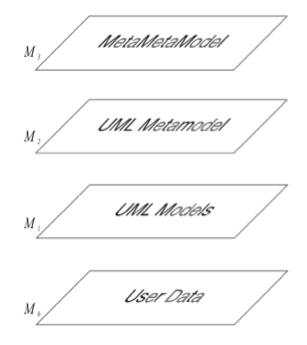
\includegraphics[width=0.4\textwidth]{images/mm_architecture.png}
\caption{The four-level meta-modeling architecture}
\label{fig:mm_architecture}
\end{figure}
The meta-meta-model (M\subscript{3}) level is the highest level, from which the UML meta-model is created. In general, it is the core from which the descriptions of specific modeling languages (i.e. specific language meta-models) are created. The UML meta-model (M\subscript{2}) describes the core from which specific language meta-models are created. Specific models are then created as instances of these language meta-models on the M1 level. The User Data depicts instances of such models created in M\subscript{1}. An example of this approach can be seen in figure ~\ref{fig:two_level_inst}.

\begin{figure}[h!]
\centering
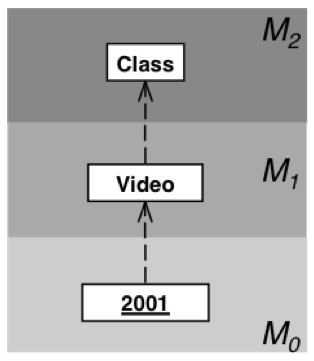
\includegraphics[width=0.4\textwidth]{images/chap2_two_level_inst.png}
\caption{Extending the two levels of instantiation}
\label{fig:two_level_inst}
\end{figure}

In this example, the dashed arrows in the figure describe an "instance of" relationship. Every level in the diagram is an instance of its level above. For example, an instantiation of the concept Video resides at level M\subscript{0}. Video on its turn is an instantiation of Class and Class is regarded as an instance of the meta-meta-model elements (the M\subscript{3} level, not shown in this example).

\subsection{Strict Meta-Modeling}

The approach described earlier exhibits a number of fundamental problems. One of them is the fact that the precise meaning of the instance-of relationship is not defined. The UML documentation does not contain a formal definition of the instance-of relationship. It merely states that a modeling level in the hierarchy must be an instance of its level above. Therefore, a formal concept should be defined to encapsulate the exact meaning of the instance-of relationship. This concept is formalized through strict meta-modeling. Strict meta-modeling states that if a model A is an instance-of another model B, then every element of A must be an instance-of some element in B \cite{RearchitectingUML}. This concept is illustrated in figure ~\ref{fig:strict_mm}. Here we see that strict meta-modeling interprets the instance-of relationship at the level of individual model elements. As a consequence, modeling levels have strict boundaries and may be crossed only by instance-of relationships.
\begin{figure}[h!]
\centering
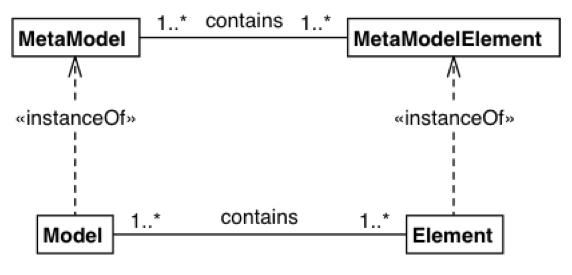
\includegraphics[width=0.7\textwidth]{images/chap2_strict_mm.png}
\caption{Strict meta-modeling.}
\label{fig:strict_mm}
\end{figure}
The exact definition of strict meta-modeling is defined as follows:
\begin{mydef}
In an \textit{n}-level modeling architecture, M\subscript{0}, M\subscript{1}, ..., M\subscript{n-1}, every element of an M\subscript{m}-level model must be an instance-of exactly one element of an M\subscript{m+1}-level model, for all \textit{m} $\leq$ \textit{m} $\le$ \textit{n-1}, and any relationship other than the instance-of relationship between two elements \textit{X} and \textit{Y} implies that level(X) = level(Y ).
\end{mydef}
It is clear that the topmost level \textit{n} is ignored in this definition. Nevertheless, we can model the top level so that its elements are instances of themselves, such that we can terminate the hierarchy of meta-levels.

\subsection{Limitations of Strict Meta-Modeling}

There are several issues with the existing UML modeling framework, such as \textit{dual classification} and the \textit{class/object duality} \cite{RearchitectingUML}. The class/duality problem arsis from the need to capture both classlike and objectlike facets of some model elements in one level and dual classification is based on the fact that we need to capture both logical (e.g. \texttt{Video}) as well as physical (e.g. \texttt{Object}) aspects of model elements. Every solution to these problems ultimately leads to unwanted, accidental complexity. They try to cramp multiple programming levels into a single modeling level, due to the limitations of strict meta-modeling. In what follows, we will focus on both the class/duality problem and the dual classification problem. For example, one could note that in figure ~\ref{fig:two_level_inst}, the M\subscript{2} level aims to address two concerns. This problem is denoted in figure ~\ref{fig:multiple_class_mm}. Here, user types at the M\subscript{0} level are defined as instances of two concepts. First, the \textit{2001} instance is an instance of the M\subscript{1}-level type \textit{Video}, and second of the M\subscript{2}-level meta-type Object. Although this approach feels natural, it is clearly in violation with our definition of strict meta-modeling:

\begin{itemize}
\item{Object 2001 has more than one classifier (Video and Object).}
\item{An instance-of relationship crosses more than one meta-level boundary.}
\end{itemize}

\begin{figure}[h!]
\centering
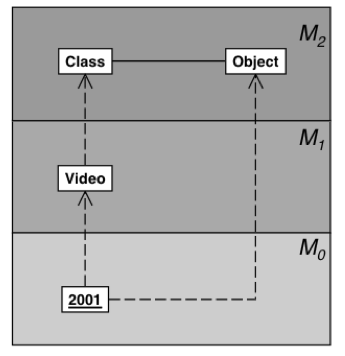
\includegraphics[width=0.4\textwidth]{images/chap2_multiple_class_uml.png}
\caption{Multiple classification in the current UML framework.}
\label{fig:multiple_class_mm}
\end{figure}

It is clear that we have to modify our approach to strict meta-modeling. The following section addresses the issues in which accidental complexity occurs and provides well-defined solutions for them.

\section{Problems with the two-level UML Modeling approach}

In this section, we will introduce an example domain model. We will also demonstrate a few workarounds used to represent multi-level domain models using only two modeling levels.

\subsection{Example domain model}

This sample model adopts a computer hardware product hierarchy using the "Item Description" pattern. This example exhibits a typical technique which is often used to capture a multi-level domain classification into the two-level UML modeling style. The example class diagram is depicted in figure ~\ref{fig:cd_itemdesc}.
\begin{figure}[h!]
\centering
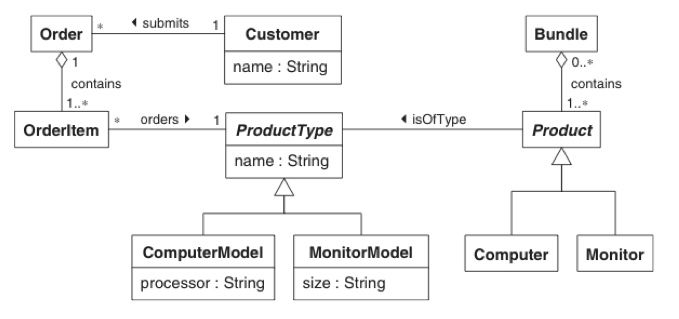
\includegraphics[width=0.9\textwidth]{images/chap2_cd_itemdesc.png}
\caption{Example class diagram of the Item Description pattern.}
\label{fig:cd_itemdesc}
\end{figure}
The above class diagram is separated into two parts. One part models products sold by an enterprise and the other part models the descriptions of these products. Here, instances of \texttt{ProductType} (\texttt{ComputerModel} and \texttt{MonitorModel}) are descriptions of the \texttt{Product} types (Computer and Monitor). The idea is to let objects play the role of classes in order to explicitly represent class-level information \cite{AccidentalComplexity}. In this way, we can dynamically change information about a product and keep this information even when no representation of this product type exists. When we create an instance of the above class diagram, we get something as depicted in figure ~\ref{fig:domain_instance}.
\begin{figure}[h!]
\centering
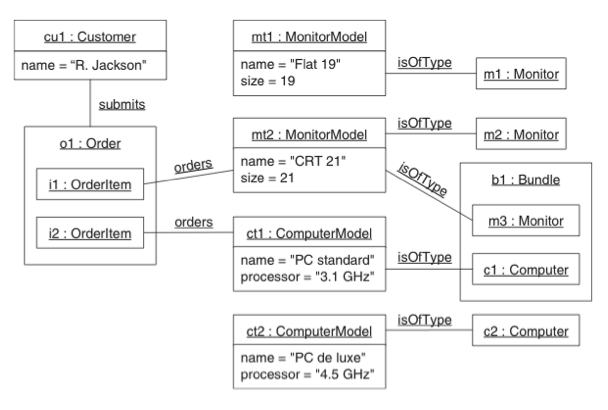
\includegraphics[width=0.9\textwidth]{images/chap2_domain_instance.png}
\caption{Domain instance (object diagram).}
\label{fig:domain_instance}
\end{figure}
The \texttt{isOfType} links between \texttt{Monitor} / \texttt{Computer} instances and \texttt{MonitorModel} / \texttt{ComputerModel} instances conceptually represent a form of \textit{instance-of} relationship (as explained in previous section), although all objects involved in the example are at the instance level in an object diagram. This verbosity does not violate strict meta-modeling, but introduces a workaround at the object level in order to create new objects at runtime.

\subsection{Domain types as objects}

We have used the graphical \texttt{isOfType} links to model the instance/type relationships at the object level. However, we can distinct up to three different kinds of instance-of relationships:

\begin{itemize}
\item{the UML built-in \textit{instance-of} relationship between the elements in the object diagram and the elements in the class diagram (e.g. \texttt{m1} \textit{instance-of} \texttt{Monitor})}
\item{the \texttt{isOfType} associations in the class diagram between \texttt{Product} classes and \texttt{ProductType} classes (e.g. \texttt{Computer} \textit{isOfType} \texttt{ComputerModel})}
\item{the \texttt{isOfType} links between instances of \texttt{Product} and instances of \texttt{ProductType} (e.g. \texttt{c2} \textit{isOfType} \texttt{ComputerModel})}
\end{itemize}
Undoubtedly, the combination of these relationships introduce some kind of accidental complexity. To see the consequences caused by this approach, we have combined the object and class diagram in one figure that explicitly represents all the relationships that conceptually exist. This diagram can be found in figure ~\ref{fig:class_object_diagram}. This figure actually highlights two aspects of the two-level modeling paradigm that was not explicitly clear from the separate diagrams:

\begin{itemize}
\item{It shows all UML \textit{instance-of} relationships explicitly in addition to the \texttt{isOfType} relationships.}
\item{It highlights the fact that the object diagram contains model information that represents domain instances and types of the domain conceptualization.}
\end{itemize}
The black dots in the figure below the dashed lines represent the domain entities. On the one hand, we have got domain types and on the other hand, we have got domain instances. The relationships between the domain entities use the same \textit{instance-of} relationships as between the model types and model instances. They represent \textit{ontological} \textit{instance-of} relationships, because they show which domain entities are considered to be types of other domain entities.
\begin{figure}[h!]
\centering
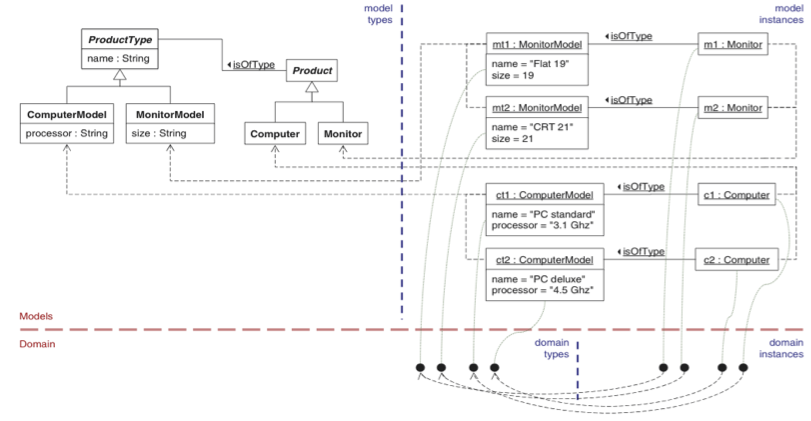
\includegraphics[width=1.0\textwidth]{images/chap2_class_object_diagram.png}
\caption{Combination of the class and object diagram.}
\label{fig:class_object_diagram}
\end{figure} \\
After investigation of the figure above, we see that it contains some redundant information. There are some model elements that do not represent any domain elements. Type \texttt{Product} and its subclasses can be considered as abundant model attributes if the model is interpreted as a domain model, because they have two classification relationships instead of just one. The subclasses \texttt{Computer} and \texttt{Monitor} merely exist to set up the \textit{Item Description} pattern. For instance, \texttt{m1} has type \texttt{Monitor} plus a modeled type \texttt{mt1}. The redundancy introduced here is an example of accidental complexity, because some information only exists to realize some workaround technique.

\subsection{Domain types as classes}

The model presented in the previous subsection is often used when we need to introduce new types of products dynamically. When we do not need to create objects dynamically at runtime, we can simplify the model significantly. This approach is shown in figure ~\ref{fig:types_classes}. It shifts some modeling elements that represent domain types (i.e. \texttt{mt1}) to the type level (into the class diagram). According to the UML class/object modeling conventions, this is a more natural place for these elements to be.
\begin{figure}[h!]
\centering
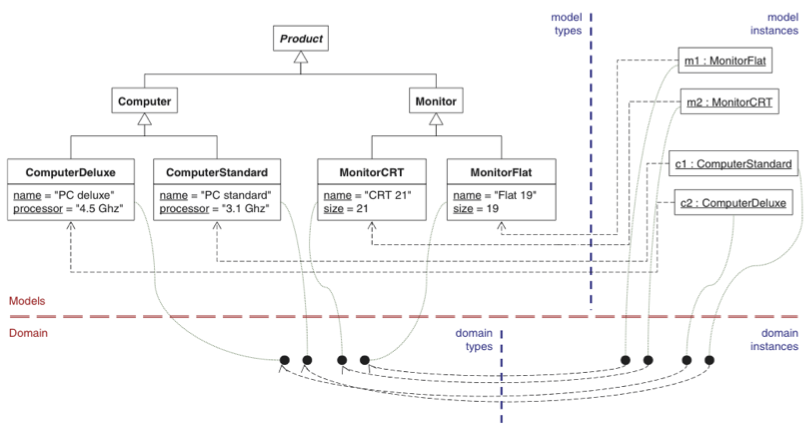
\includegraphics[width=1.0\textwidth]{images/chap2_types_classes.png}
\caption{Types as classes.}
\label{fig:types_classes}
\end{figure} \\
Although the figure above removes some accidental complexity from the previous example, we also lost some features. It is no longer possible to instantiate new types at runtime, because product types are now represented by classes. Without additional information, we cannot conclude whether the workaround methods of previous section were necessary or not. Therefore, it is hard to compare the models and evaluate them on the level of accidental complexity. In the next chapter we will see whether it is possible to keep the simplicity of figure ~\ref{fig:types_classes} and still support the ability to create new product types at runtime.
